\documentclass[t]{beamer}

\ifluatex
\usepackage[utf8]{luainputenc}
\else
\usepackage[utf8]{inputenc}
\usepackage[T1]{fontenc}
\fi

\usepackage[ngerman]{babel}

\usepackage[]{blindtext}

\title{Das neue \LaTeX-Beamer Theme der TU~Dortmund}
\author{Maximilian Nöthe}
\institute[Lehrstuhl E5b \\ Fakultät Physik]{Lehrstuhl E5b \par\vspace{3pt} Fakultät Physik}
\titlegraphic{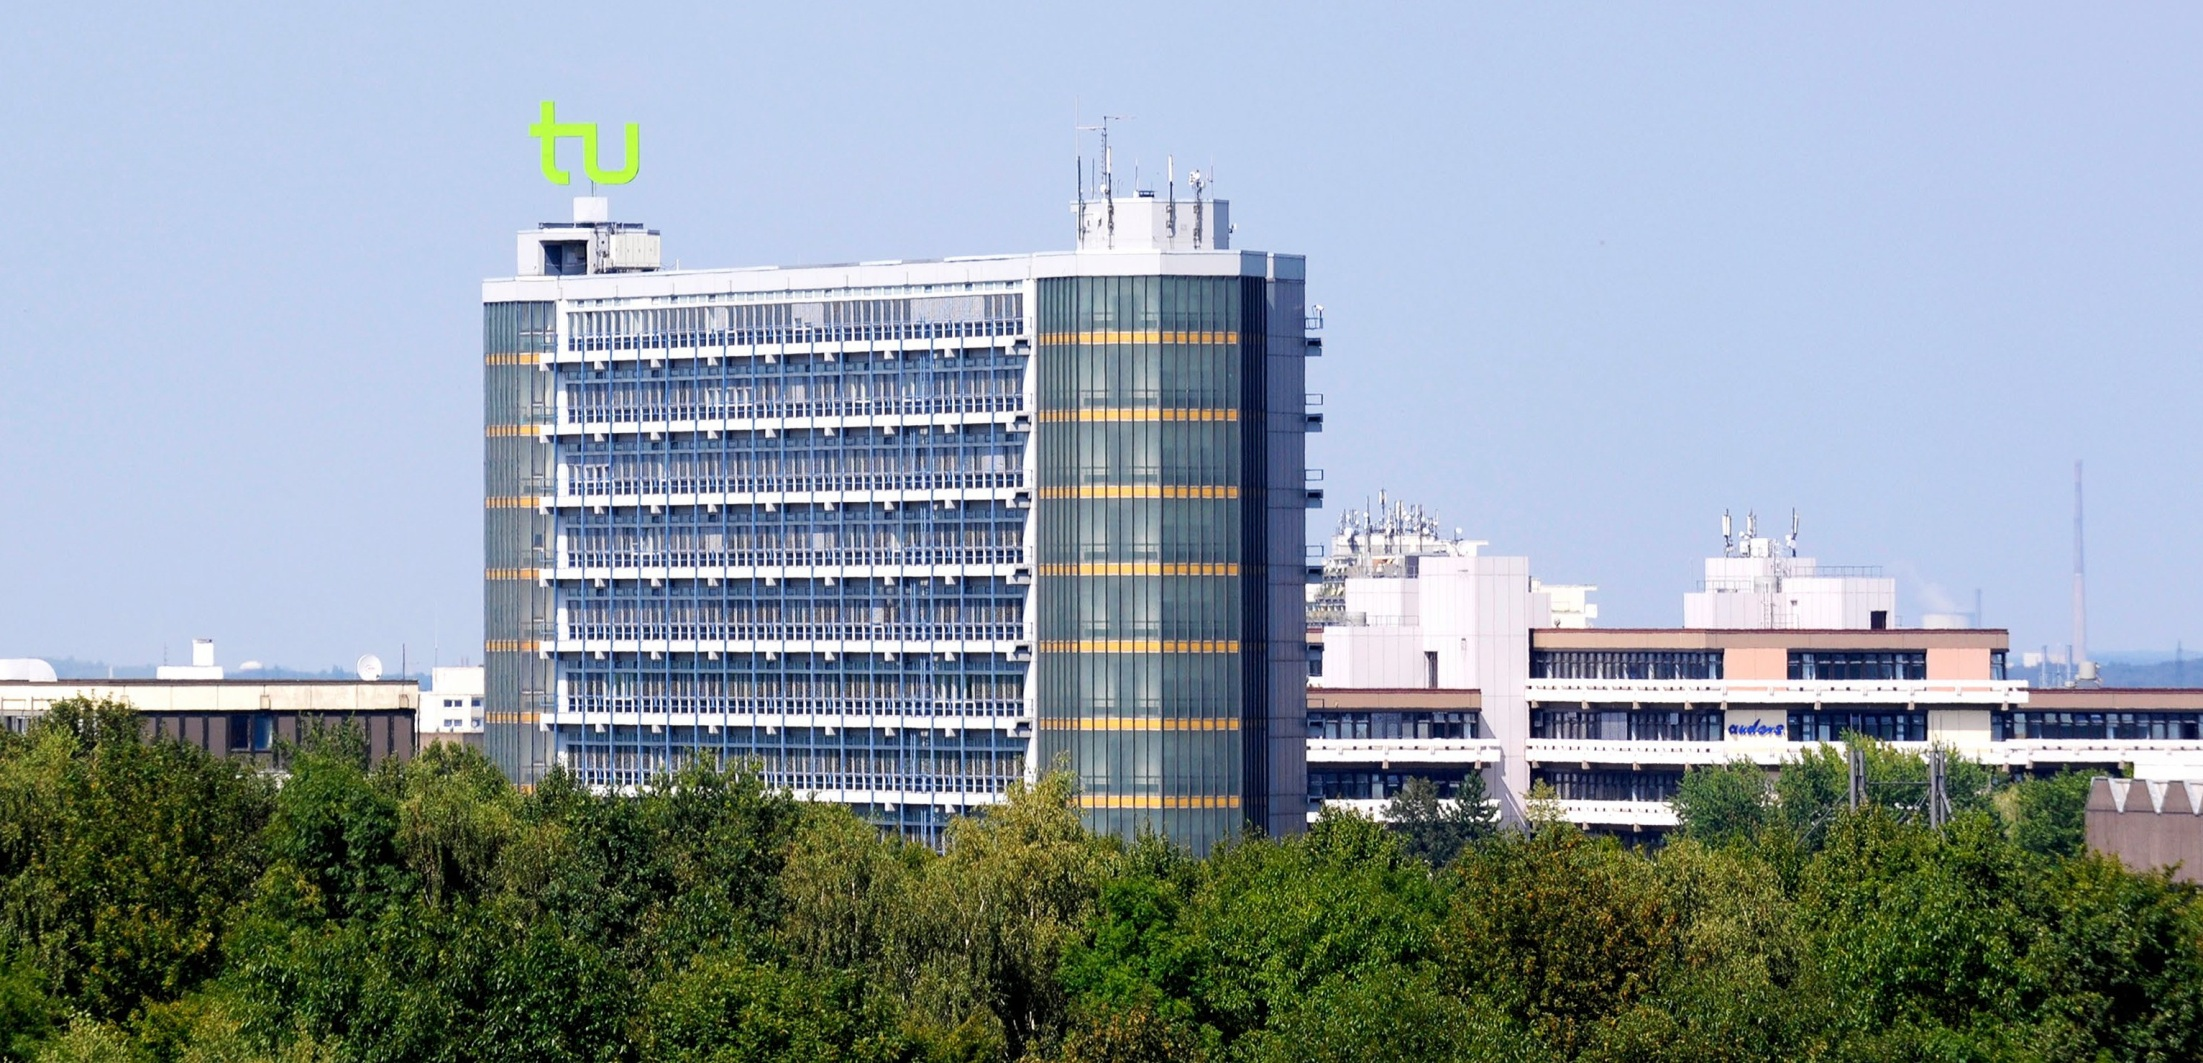
\includegraphics[height=0.7\textheight]{Title-Pic.jpg}}

\usetheme{TUDo}

\begin{document}

\begin{frame}
\setcounter{framenumber}{0}
    \titlepage
\end{frame}

\begin{frame}
    \frametitle{Einführung}
    \tableofcontents[pausesections]
\end{frame}

\section{Das Design}
\subsection{Farben und Formen}
\begin{frame}
    \frametitle{Die TU-Farbpalette}
    \framesubtitle{herbstlich}
    \begin{itemize}
        \item \textcolor{TUgreen}{TUgreen}
            \begin{itemize}
                \item \textcolor{TUlightgreen}{TUlightgreen}
                \item \textcolor{TUdarkgreen}{TUdarkgreen}
                \item \textcolor{TUolive}{TUolive}
            \end{itemize}
        \item \textcolor{TUyellow}{TUyellow}
        \item \textcolor{TUcitron}{TUcitron}
        \item \textcolor{TUlime}{TUlime}
        \item \textcolor{TUorange}{TUorange}
    \end{itemize}
\end{frame}

\subsection{Blöcke}
\begin{frame}
    \frametitle{Blöcke}
    \begin{block}{block}
        \begin{itemize}
            \item 1
            \item 2
        \end{itemize}
    \end{block}
    \begin{alertblock}{alertblock}
        \begin{itemize}
            \item 1
            \item 2
        \end{itemize}
    \end{alertblock}
    \begin{exampleblock}{exampleblock}
        \begin{itemize}
            \item 1
            \item 2
        \end{itemize}
    \end{exampleblock}
\end{frame}

\section{Beispiel-Slides}
\subsection{Mehrspaltige Slides}
\begin{frame}{zweispaltiges Layout}
    \begin{columns}
        \begin{column}{0.49\textwidth}
            \begin{block}{Block 1}
                Test
            \end{block}
            \begin{block}{Block 2}
                Test
            \end{block}
        \end{column}
        \begin{column}{0.49\textwidth}
            \begin{itemize}
                \item Test 1
                \item Test 2
                \item Test 3
            \end{itemize}
        \end{column}
    \end{columns}
\end{frame}

\begin{frame}{zweispaltiges Layout}{mit Bild}
    \begin{columns}[T] % Use [T]-Option to align images at top border
        \begin{column}{0.49\textwidth}
            \begin{itemize}
                \item super Mathe-Tower
                \item super TU-Logo
                \item super Physik-Gebäude
                \item super geil
            \end{itemize}
        \end{column}
        \begin{column}{0.49\textwidth}
            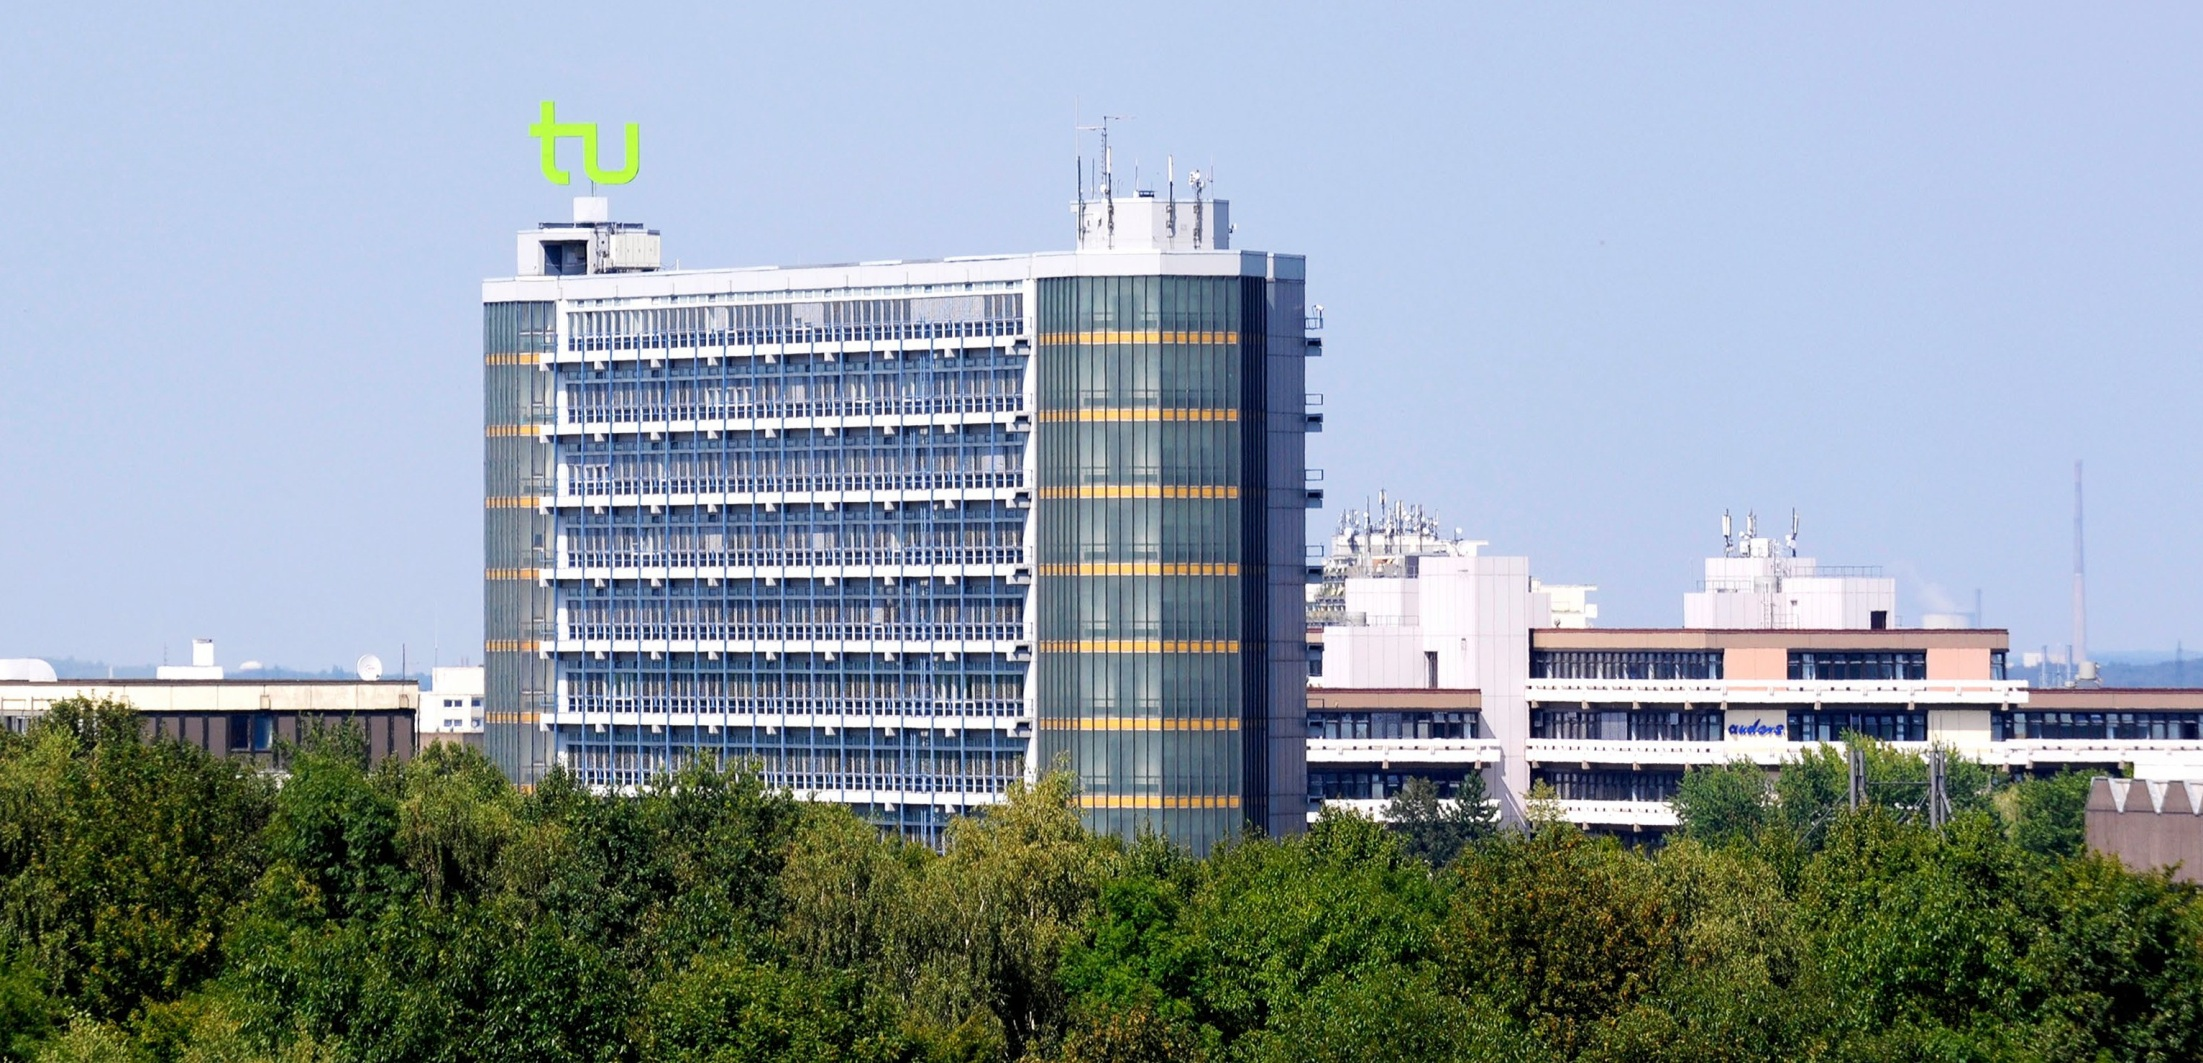
\includegraphics[width=\textwidth]{./Title-Pic.jpg}\\
        \end{column}
    \end{columns}
    \vspace{5pt}%
    \begin{columns}[T] % Use [T]-Option to align images at top border
        \begin{column}{0.49\textwidth}
            \hfill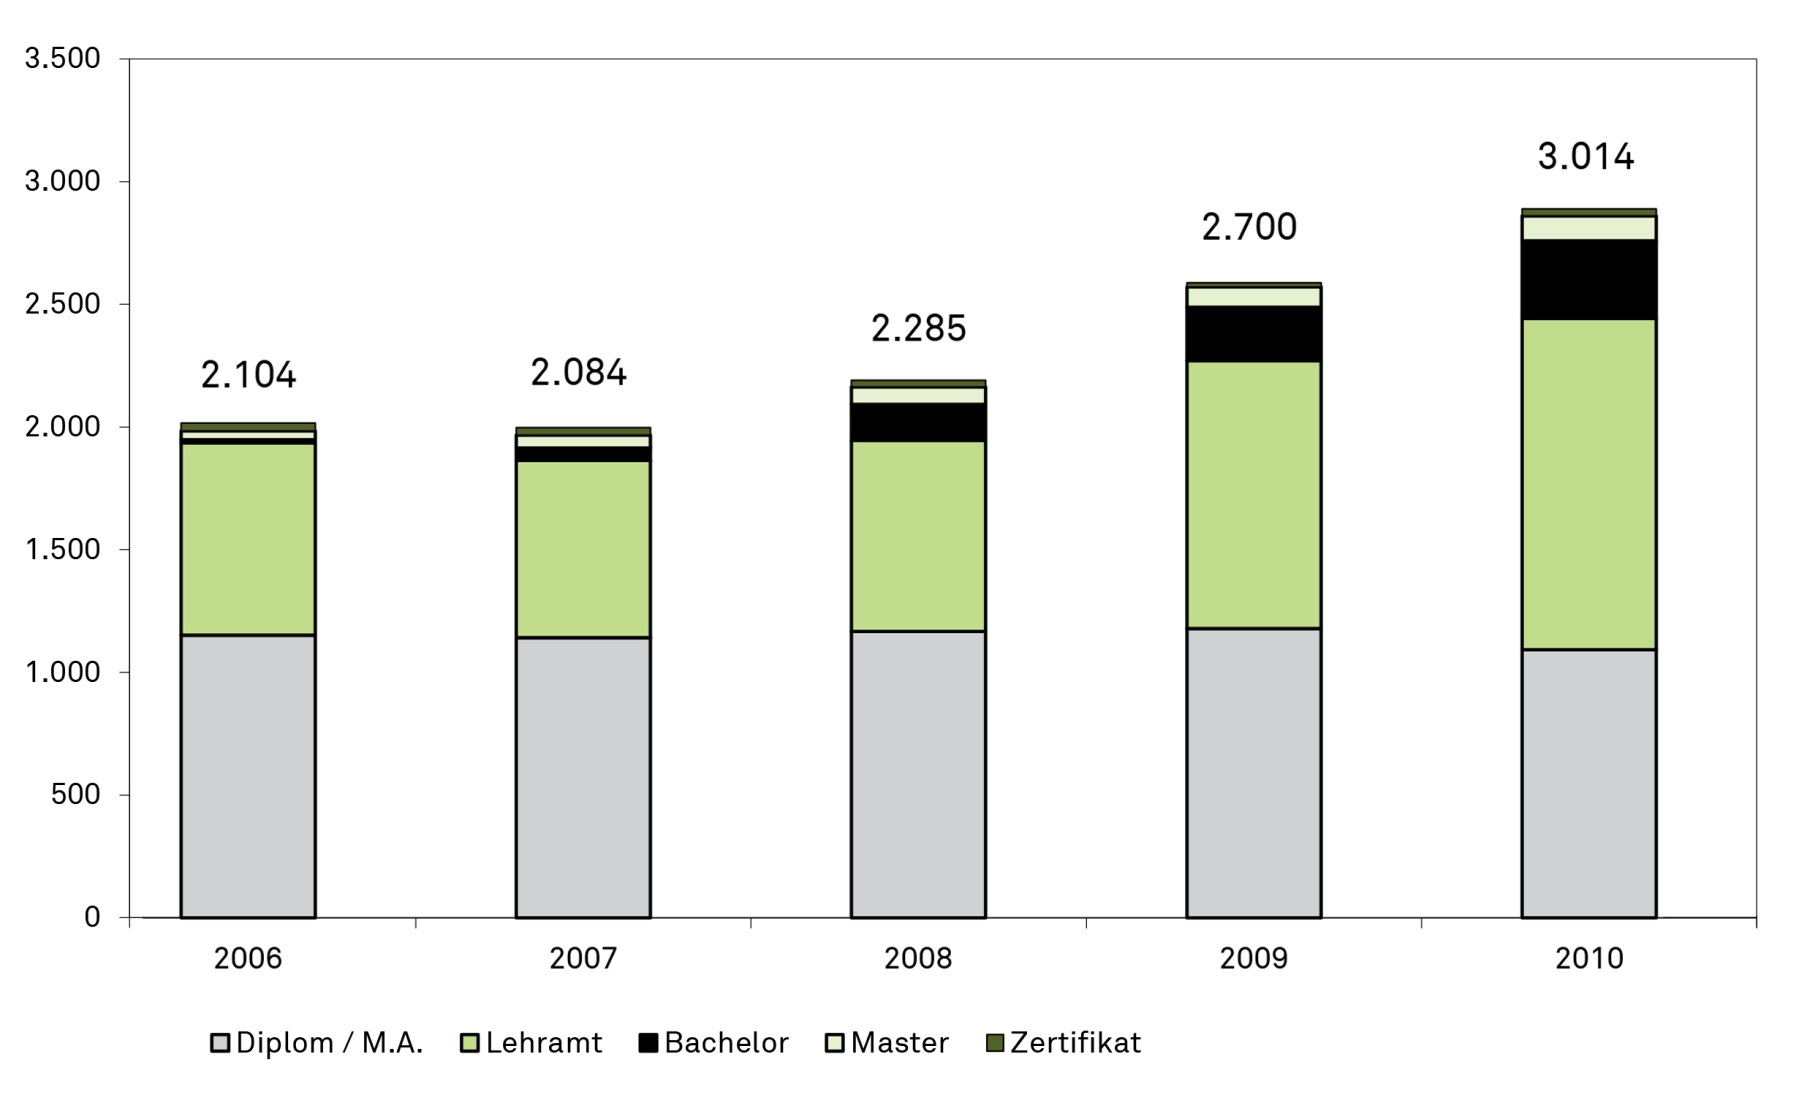
\includegraphics[width=\textwidth]{./image23.jpg}
        \end{column}
        \begin{column}{0.49\textwidth}
            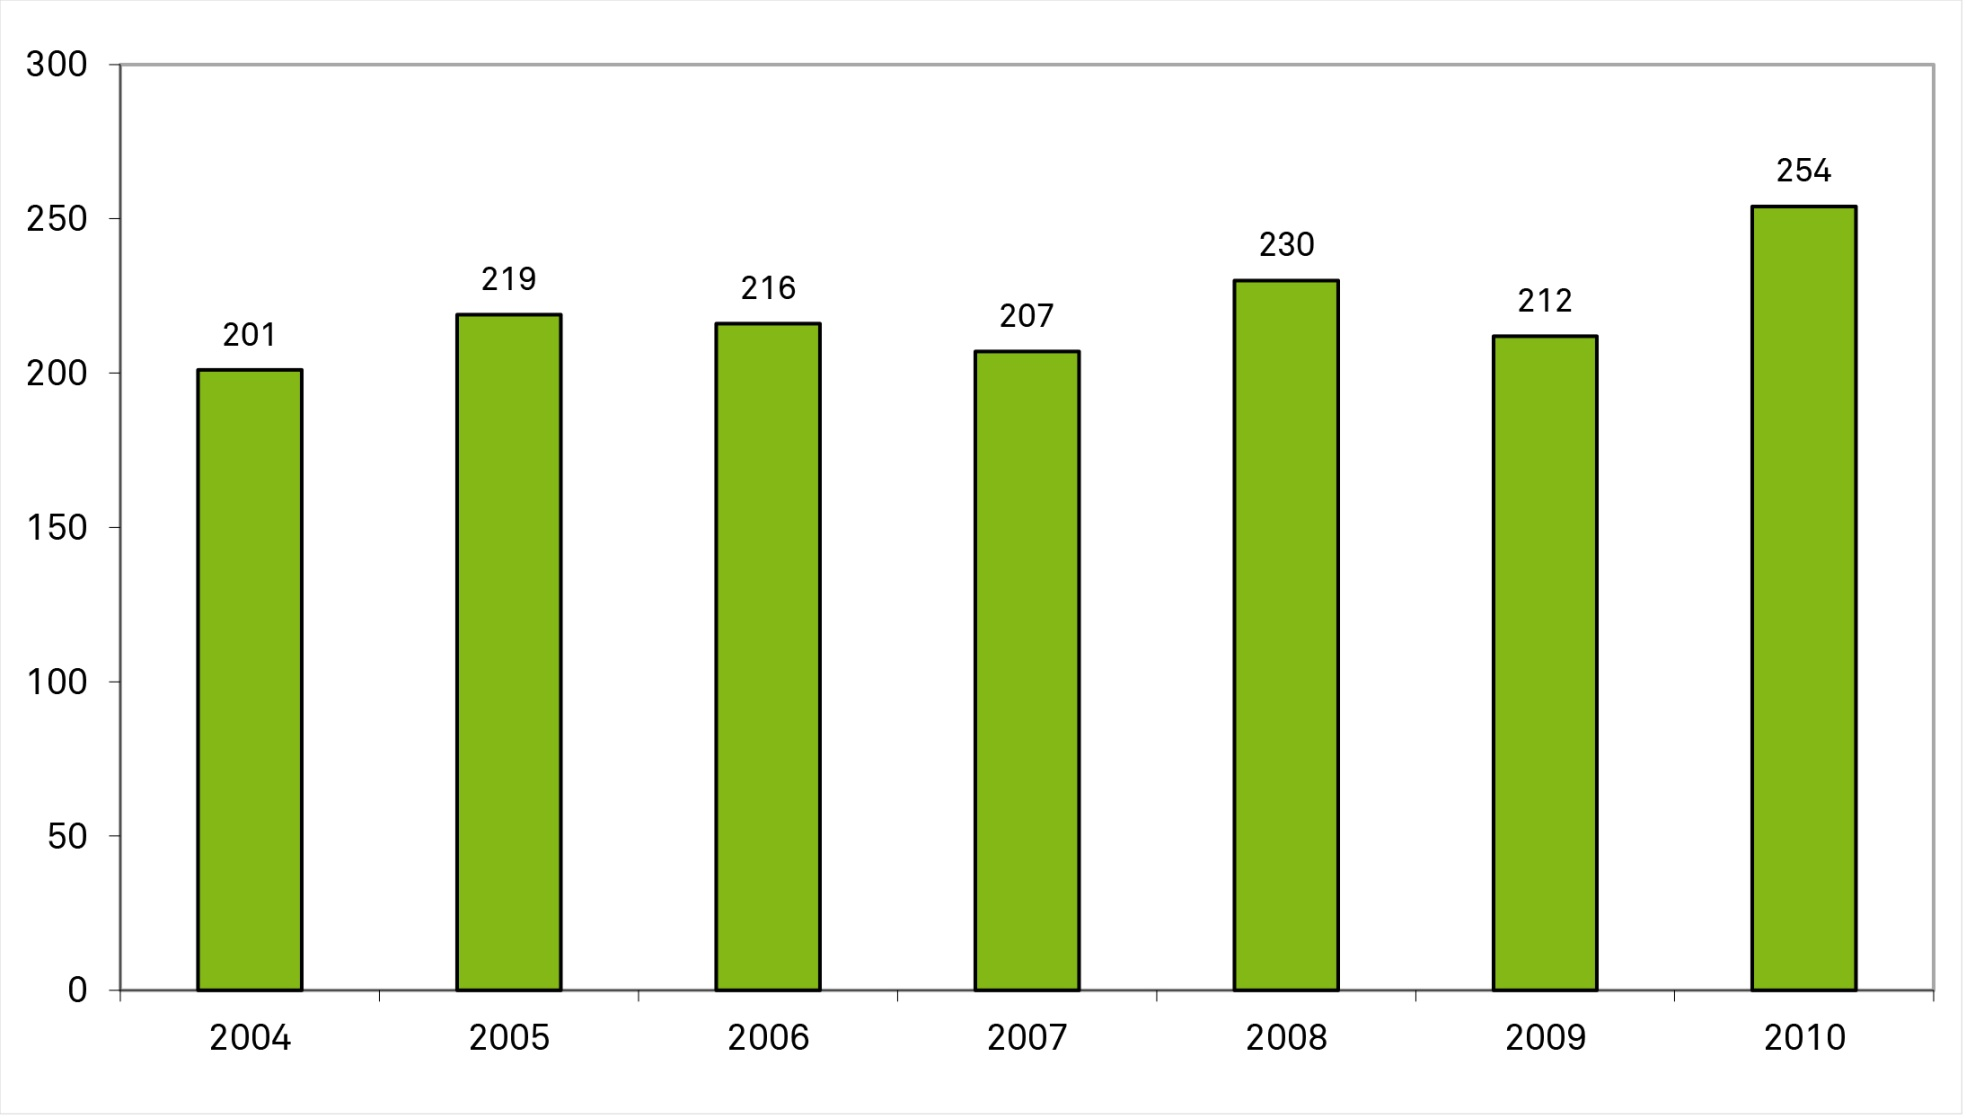
\includegraphics[width=\textwidth]{./image24.jpg}
        \end{column}
    \end{columns}
\end{frame}
\end{document}
